\documentclass[12pt]{beamer}
\usetheme{Copenhagen}
\usepackage[utf8]{inputenc}
%\usepackage[spanish]{babel}
\usepackage[spanglish]{babel}
\usepackage{amsthm,amsmath,amsfonts,amssymb}
\usepackage{graphicx}
\usepackage{subcaption}
\usepackage{threeparttable}
\usepackage{multicol}


\newcommand\Wider[2][3em]{%
\makebox[\linewidth][c]{%
  \begin{minipage}{\dimexpr\textwidth+#1\relax}
  \raggedright#2
  \end{minipage}%
  }%
}


\newtheorem{definic}{Definición}[section]
\newtheorem{teorema}{Teorema}[section]
\title{Estimación de Tipo de Cambio Real de Equilibrio para Bolivia}
\author{Hugo Pablo Rocha Portugal \and Paola Yujra Tonconi}
\date{\today}
\begin{document}

\begin{frame}
\titlepage
\end{frame}

\begin{frame}{Agenda}
\begin{multicols}{2}
%\tiny
\tableofcontents
\end{multicols}
\end{frame}

\section[Introducción]{Introducción}

\begin{frame}{Objetivos}
\begin{itemize}
\item Qué es el tipo de cambio real de equilibrio
\item Modelos mainstream con datos de Bolivia
\item Consideraciones heterodoxas 
\item Consideraciones de política económica
\end{itemize}
\end{frame}

\section[Marco teórico]{Marco teórico}

\begin{frame}{Definiciones}
\begin{definic}[Tipo de cambio real]
\begin{equation}\label{tcr1}
Q_t=E_t\frac{P_t^*}{P_t},
\end{equation}
\begin{equation}\label{tcrlog}
q_t=e_t+p_t^*-p_t.
\end{equation}
\end{definic}
Si $p_t=\alpha p_{Nt} + (1-\alpha) p_{Tt}$, $0<\alpha<1$ y $\alpha=\alpha^*$
\begin{equation}\label{tcr2}
q_t=q_{Tt}+\alpha(\hat{p}_{Nt}-\hat{p}_{Tt}),
\end{equation}
donde: $\hat{p}_{\bullet t}=p_{\bullet t}^*-p_{\bullet t}$ y $q_{Tt}=e_{Tt}+p_{Tt}^*-p_{Tt}$.
\end{frame}

\subsection[Definiciones]{Definiciones}

\begin{frame}
\begin{definic}[Tipo de cambio real de equilibrio]
Es una variable no observada que determina los valores  ``económicamente ideales" del tipo de cambio real.
\end{definic}
Consideraciones
\begin{itemize}
\item Qué es ``económicamente ideales" depende de la perspectiva por la cual se defina.
\item Contrafactual del tipo de cambio real.
\item Implica el equilibrio de los mercados de la economía y economías adyacentes?
\end{itemize}
\end{frame}

\begin{frame}
\Wider{\begin{equation}
q_t=\beta'Z_t+\theta'T_t+\varepsilon_t
\end{equation}
\begin{itemize}
\item $q_t^{cp}=\beta'Z_t+\theta'T_t$.\\
No toma en cuenta shocks inesperados.
\item $\hat{q}_t=\beta'\hat{Z}_t$.\\
No toma en cuenta shocks inesperados ni shocks transitorios y los fundamentos están a un nivel tendencial.
\item $q_t^{lp}=\beta'\bar{Z}_t$.\\
No toma en cuenta shocks inesperados ni shocks transitorios y los fundamentos están en \emph{steady state} o su nivel de largo plazo.
\end{itemize}
}
\end{frame}

\subsection[Métodos]{Métodos}

\begin{frame}{Métodos}
\begin{itemize}
\item[CP] UIP, Modelos Monetarios, CHEER, ITMEER, BEER, SVAR, DSGE.
\item[MP] FEER, DEER, APEER, PEER.
\item[LP] PPP, Balassa-Samuelson, APEER, PEER, NATREX, SVAR, DSGE.
\end{itemize}
Entonces, queremos determinar si el tipo de cambio real efectivamente puede lograr un equilibrio en balanza de pagos y cuales son los fundamentos del tipo de cambio real.
\end{frame}

\subsection[Consideraciones]{Consideraciones}

\begin{frame}{Consideraciones}
\Wider{
\begin{itemize}
\item \emph{Steady state} no es pertinente en las economías de desarrollo.
\item Los modelos de corto plazo determinan el comportamiento del TCR a través del movimiento de los fundamentos. La bibliografía sobre la aplicación boliviana se basa en modelos reducidos de cointegración que carecen de una adecuada identificación teórica.
\item Los modelos de mediano plazo están basados en un balance interno y externo caracterizados por un equilibrio general o parcial determinando por un objetivo claro de política.
\end{itemize}}
\end{frame}

\section[Metodología]{Metodología}
\subsection[BEER clásico]{BEER clásico}
\begin{frame}{Identificación BEER clásico}
\Wider{\begin{definic}[Paridad de tasa de interés encubierta]
\begin{equation}
\mathbb{E}_t[\Delta e_{t+k}]=-(i_t-i_t^*)+\pi_t,
\end{equation}
\end{definic}
\begin{equation}
q_t=\mathbb{E}_t[q_{t+k}]+(r_t-r_t^*)+\pi_t.
\end{equation}
Donde: $\pi_t=\lambda_t+k$, $\lambda_t=g(\frac{gd_t}{gd_t^*})$ y $\mathbb{E}_t[q_{t+k}]=\mathbb{E}_t[\beta' Z_t]=\beta' Z_t$. Entonces:
\begin{equation}\label{qb}
q_t=f(Z_t)+(r_t-r_t^*)+\lambda_t+k
\end{equation}}
\end{frame}

\subsection[BEER equilibrio parcial]{BEER equilibrio parcial}
\begin{frame}{Identificación BEER equilibrio parcial}
\Wider{Se utiliza el modelo de Calderón (2002,2004) quien formula una versión extendida del modelo original de transables y no transables de Obsfeld y Rogoff (1995,1996).
\begin{itemize}
\item Equilibrio parcial para dos economías, el país doméstico y el país extranjero, cada uno cuenta con un sector transable y no transable.
\item Existe un agente representativo en la economía que mantiene preferencias homotéticas.
\item Ambos países tiene un agente representativo y un productor.
\item El sector transable tiene un bien homogéneo valorado de manera competitiva en los mercados mundiales. El sector no transable es monopolista.
\end{itemize}}
\end{frame}

\begin{frame}
\begin{itemize}
\item El agente representativo del país nacional está dotado de una cantidad constante del bien transable en cada periodo $Y_t$. Asimismo, este agente tiene el poder monopólico sobre los bienes no transables $A_t$, en la economía.
\item El agente del país domestico tienen las mismas preferencias del agente extranjero, en cuanto a sus decisiones de consumo, ahorro y esfuerzo laboral.
\item El gasto de gobierno se direcciona principalmente a bienes no transables, lo que ejerce una presión sobre la demanda de los mismos.
\item El gasto de gobierno es puramente dispersa y no afectan a la productividad o utilidades privadas.
\item Por simplicidad se asume que el consumo doméstico y el de gobierno en bienes exportables es cero.
\end{itemize}
\end{frame}

\begin{frame}
\Wider{Si:
\begin{equation}
C_t=[\gamma^{\frac{1}{\theta}}C_{Tt}^{\frac{\theta-1}{\theta}}+(1-\gamma^{\frac{1}{\theta}})C_{Nt}^{\frac{\theta-1}{\theta}}]^{\frac{\theta}{\theta-1}}
\end{equation}
\begin{equation}
P_t=[\gamma P_{Tt}^{1-\theta}+(1-\gamma)P_{Nt}^{1-\theta}]^{\frac{1}{1-\theta}}
\end{equation}
Entonces se maximiza la utilidad del agente $j$:
\begin{equation}
\max_{C_t,F_{s+1}^j} U_t^j= \max_{C_t,F_{s+1}^j} \sum_{s=t}^\infty \beta^{s-t} \left[\frac{\sigma}{\sigma -1}C_s^{\frac{\sigma -1}{\sigma}}-\frac{\kappa}{2}Y_{Ns}^2\right]
\end{equation}
\begin{equation}
s.t.\quad F_{t+1}^j=(1+r_t)F_{t}^j+P_{Nt}(j)Y_{Nt}(j)-P_{Tt}^X Y_{Tt}-P_tC_t^j -P_t\tau
\end{equation}}
\end{frame}

\begin{frame}
Con la finalidad de introducir al gobierno, se asume que el gasto de gobierno es puramente disipativa y no afecta a la productividad o utilidades privadas. Por lo tanto los productores de no transables tienen una curva de demanda con pendiente descendente desde el sector público y privado.
\begin{equation}
Y_{Nt}^D(j)=\left[ \frac{P_{Nt}(j)}{P_{Nt}} \right]^{-\theta}C_N^A
\end{equation}
\begin{equation}
G_{t}(j)=\left[ \frac{P_{Nt}(j)}{P_{Nt}} \right]^{-\theta}G_N^A
\end{equation}
\end{frame}

\begin{frame}
\Wider{Solución log linealizada del modelo:
\begin{equation}
\tilde{Y}_N=\tilde{C}_N=\left(\frac{\sigma-\theta}{\sigma-1}\right)\gamma(\tilde{P}_N-\tilde{P}_T)+\left(\frac{\sigma}{\sigma+1}\right)\tilde{A}_N
\end{equation}
\begin{equation}
\tilde{P}_N-\tilde{P}_T=\frac{1+\sigma}{\theta(1+\sigma)+\gamma(\sigma-\theta)}\left[ r\tilde{F}+\tilde{Y}_T+\tilde{P}^X_T-\frac{\sigma}{1+\sigma}\tilde{A}_N+\tilde{G} \right]
\end{equation}
\begin{align}
\tilde{P}_N^*-\tilde{P}_T^*=&\frac{1+\sigma}{\theta(1+\sigma)+\gamma(\sigma-\theta)}\left[-\left(\frac{n}{1-n}\right) r\tilde{F}+\tilde{Y}_T^*+\tilde{P}^M_T\right. \\ \nonumber
& \left.-\frac{\sigma}{1+\sigma}\tilde{A}_N^*+\tilde{G}^* \right]
\end{align}}
\end{frame}

\begin{frame}
\Wider{Incorporando las ecuaciones a la ecuación de tipo de cambio real
\begin{align}
\tilde{q}_t=&\tilde{e}_t+(\tilde{P}_{T}^*-\tilde{P}_{T})+\psi r\tilde{F}\left(\frac{1}{1-n}\right)+\psi (\tilde{Y}_{T}-\tilde{Y}_{T}^*)\\\nonumber&-\left(\psi\frac{\sigma}{1+\sigma}\right)(\tilde{A}_N-\tilde{A}_N^*)+\psi(\tilde{G}-\tilde{G}^*)+\xi
\end{align}
\begin{align}
\ln TCR_t=&\phi_0+\phi_1\left(\frac{F}{Y}\right)_t+\phi_2\ln\left(\frac{Y_T}{A_N} / \frac{Y_T^*}{A_N^*}\right)_t+\phi_3\ln\left(\frac{P_T^X}{P_T^M}\right)_t\\\nonumber&+\phi_4\ln\left(\frac{G}{G^*}\right)_t+O+\mu_t
\end{align}
Donde $O$ son otras variables de control.}
\end{frame}

\begin{frame}{Fundamentos}
\Wider{\begin{itemize}
\item Coeficiente de la posición de activos externos netos: Obstfed y Rogoff (1998) y Lane y Milesi-Ferreti (2004): Países con pasivos externos importantes (deudores netos) necesitan generar un superávit en la balanza comercial, para poder honrar sus deudas lo que obliga a una depreciación.
\item La productividad laboral del sector transable entre el país doméstico y el foráneo: un incremento de la productividad en el sector transable en el país doméstico respecto a la del país foráneo originaran una apreciación del TCR (bienes transables son homogéneos y están valorados de manera homogénea)
\item Términos de intercambio: Efecto es teóricamente indefinido, debido a al efecto ingreso y sustitución
\end{itemize}}
\end{frame}

\begin{frame}
\begin{itemize}
\item Gasto de gobierno como proporción del PIB: Supuesto se destina a bienes no transables, por lo que toda presión del gasto público sobre este sector causa un exceso de demanda y posteriormente una subida del precio de bienes no transables, dando como resultado una apreciación real.
\end{itemize}
Otras variables:
\begin{itemize}
\item Equilibrio interno: Desempleo
\item Política comercial: 
\item Impuesto a las importaciones
\item Apertura comercial
\end{itemize}
\end{frame}

\subsection[DEER]{DEER}
\begin{frame}{Identificación}
\begin{definic}[Cuenta Corriente]
\begin{equation}\label{CC}
CC\equiv(P_XX-P_MM)+Ing1+Ing2
\end{equation}
\begin{equation}\label{cc}
cc=\frac{CC}{PIB}=\frac{BC}{PIB}+\frac{Ing1}{PIB}+\frac{Ing2}{PIB}
\end{equation}
\end{definic}
\begin{equation}\label{sup}
\frac{\partial CC}{\partial Q}=\frac{\partial BC}{\partial Q}
\end{equation}
Suponiendo $\frac{\partial Ing1}{\partial Q}=0$, $\frac{\partial Ing2}{\partial Q}=0$ y $\frac{\partial CC}{\partial Q}\approx \frac{\Delta CC}{\Delta Q}=CC-\bar{CC}$
\begin{equation}\label{dc}
\frac{\partial cc}{\partial Q}=cc-\bar{cc}
\end{equation}
\end{frame}

\begin{frame}
\Wider{Si:
\begin{equation}\label{X}
X=f(\overset{+}{Y^*},\overset{+}{Q})
\end{equation}
\begin{equation}\label{M}
M=g(\overset{+}{Y},\overset{-}{Q})
\end{equation}
Entonces:
\begin{equation}
bc=\frac{P_X X}{PIB}-\frac{P_M M}{PIB}.
\end{equation}
\begin{equation}
\frac{\partial bc}{\partial Q}=\frac{\partial X}{\partial Q} \frac{P_X}{PIB}+\frac{\partial P_X}{\partial Q} \frac{X}{PIB} - \frac{\partial M}{\partial Q} \frac{P_M}{PIB}-\frac{\partial P_M}{\partial Q}\frac{M}{PIB},
\end{equation}
Donde: $\frac{\partial P_X}{\partial Q}=0$ y $\frac{\partial P_M}{\partial Q}=-\frac{P_M}{Q}$. Entonces:
\begin{equation}\label{partialq}
\frac{\partial bc}{\partial Q}=\frac{1}{Q} \left[\eta_X \frac{P_X X}{PIB}-(\eta_M -1)\frac{P_M M}{PIB}\right].
\end{equation}}
\end{frame}

\begin{frame}
\begin{equation}
\frac{\partial cc}{\partial Q}=\frac{\partial bc}{\partial Q}
\end{equation}
\begin{equation}
Q^{DEER}=\frac{1}{cc-\bar{cc}}\left[\eta_X \frac{P_X X}{PIB}-(\eta_M -1)\frac{P_M M}{PIB}\right].
\end{equation}
\end{frame}

\section[Resultados]{Resultados}
%\subsection[BEER]{BEER}


\subsection[DEER]{DEER}
\begin{frame}{Variables incluidas}
\begin{figure}
\centering
    \begin{subfigure}[b]{0.3\textwidth}
        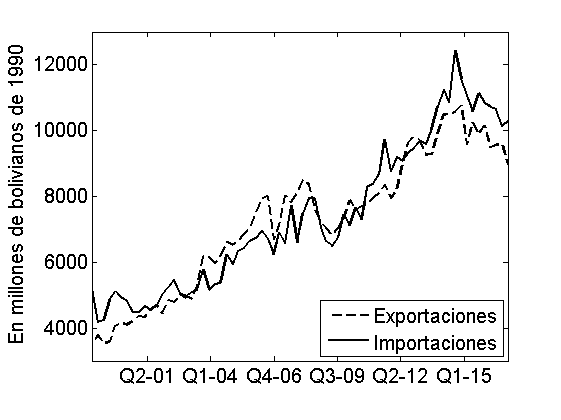
\includegraphics[width=\textwidth]{1xm}
        \caption{\tiny Exportación e importación}
        \label{1xm}
    \end{subfigure}
    ~ %add desired spacing between images, e. g. ~, \quad, \qquad, \hfill etc. 
      %(or a blank line to force the subfigure onto a new line)
    \begin{subfigure}[b]{0.3\textwidth}
        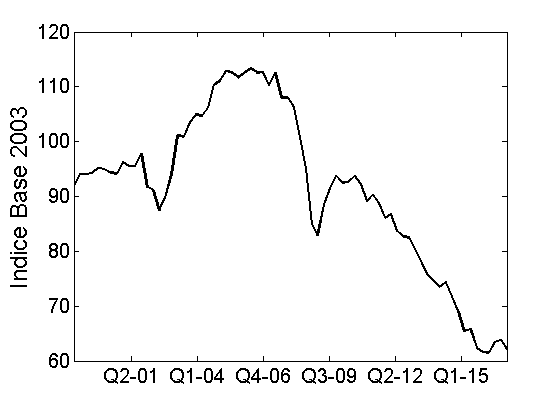
\includegraphics[width=\textwidth]{3tcr}
        \caption{\tiny TCR}
        \label{3tcr}
    \end{subfigure}
    ~ %add desired spacing between images, e. g. ~, \quad, \qquad, \hfill etc. 
    %(or a blank line to force the subfigure onto a new line)
    \begin{subfigure}[b]{0.3\textwidth}
        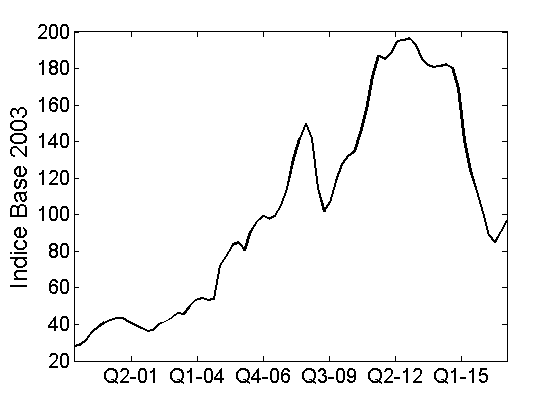
\includegraphics[width=\textwidth]{5ippbx}
        \caption{\tiny Precios internacionales}
        \label{5ippbx}
    \end{subfigure}
    \begin{subfigure}[b]{0.3\textwidth}
        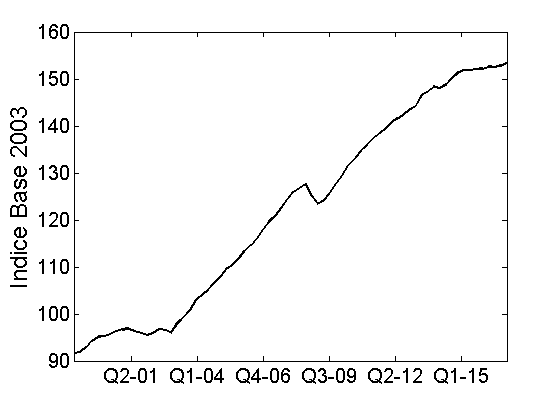
\includegraphics[width=\textwidth]{2per}
        \caption{\tiny PIB externo relevante}
        \label{2per}
    \end{subfigure}
    ~ %add desired spacing between images, e. g. ~, \quad, \qquad, \hfill etc. 
      %(or a blank line to force the subfigure onto a new line)
    \begin{subfigure}[b]{0.3\textwidth}
        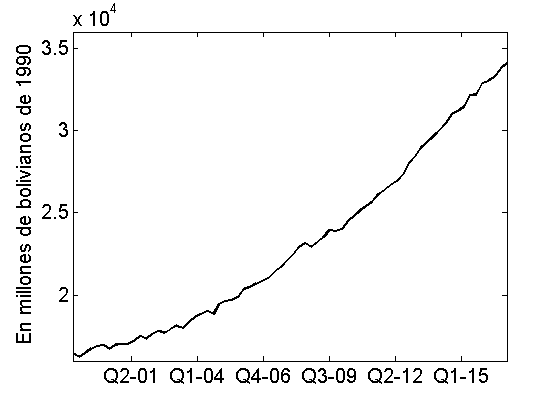
\includegraphics[width=\textwidth]{4pib}
        \caption{\tiny PIB}
        \label{4pib}
    \end{subfigure}
\end{figure}
\end{frame}

\begin{frame}{Estructura de importaciones de Bolivia}
\begin{figure}
\centering
    \begin{subfigure}[b]{\textwidth}
        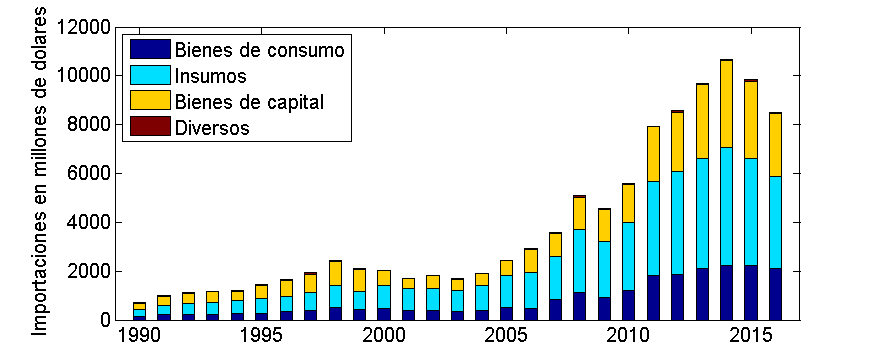
\includegraphics[width=\textwidth]{imp9016}
        \label{mestr}
    \end{subfigure}
\end{figure}
\end{frame}

\begin{frame}{Estructura de exportaciones de Bolivia}
\begin{figure}
\centering
    \begin{subfigure}[b]{\textwidth}
        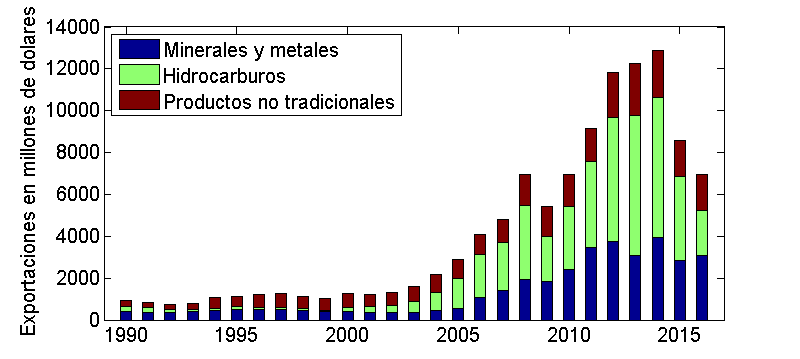
\includegraphics[width=\textwidth]{exp9016}
        \label{xestr}
    \end{subfigure}
\end{figure}
\end{frame}

\begin{frame}{Matriz de correlación}
\begin{table}
\begin{center}
\begin{threeparttable}
\scalebox{0.6}{
\begin{tabular}{lcccccc}									
\hline													
\hline												
	&	Exportaciones	&	Importaciones	&	PIB externo	&	TCR	&	IPPBX	&	PIB	\\
\hline													
Exportaciones	&	1	&		&		&		&		&		\\
Importaciones	&	0.9384	&	1	&		&		&		&		\\
PIB externo	&	0.9424	&	0.9751	&	1	&		&		&		\\
TCR	&	-0.5185	&	-0.7131	&	-0.7103	&	1	&		&		\\
IPPBX	&	0.8949	&	0.8506	&	0.8743	&	-0.3589	&	1	&		\\
PIB	&	0.9017	&	0.9645	&	0.9835	&	-0.8102	&	0.7821	&	1	\\
\hline													
\hline									
\end{tabular}	
}						
\begin{tablenotes}
\small
\item Elaboración propia.
\end{tablenotes}	
\end{threeparttable}
\end{center}
\end{table}	
\end{frame}

\begin{frame}{Ecuaciones de comercio}
\begin{table}
\begin{center}
\begin{threeparttable}
\scalebox{0.7}{
\begin{tabular}{lcccc}									
\hline									
\hline	
	&	(1)	&	(2)	&	(3)	&	(4)	\\
	&	$x$	&	$\Delta x$	& $m$	&	$\Delta m$	\\
\hline	
$y^*$	&	1.700***	&		&		&		\\
	&	(0.035)	&		&		&		\\
$\Delta y^*$	&		&	1.135*	&		&		\\
	&		&	(0.626)	&		&		\\
$y$	&		&		&	1.008***	&		\\
	&		&		&	(0.020)	&		\\
$\Delta y$	&		&		&		&	1.018	\\
	&		&		&		&	(0.353)	\\
$tcr$	&	0.155***	&	&	-0.276***	&	\\
	&	(0.037)	&	&	(0.044)	&	\\
$\Delta tcr$	&	&	0.499**	&	&	-0.095	\\
	&	&	(0.212)	&	&	(0.075)	\\
\hline									
\hline									
\end{tabular}
}	
\begin{tablenotes}
\small
 \item  \emph{Nota.} La significancia al uno, cinco y diez por ciento es indicada por ***, ** y *, respectivamente.
\end{tablenotes}								
\end{threeparttable}					
\end{center}
\label{Rec}	
\end{table}	
\end{frame}

\begin{frame}
\begin{figure}
\centering
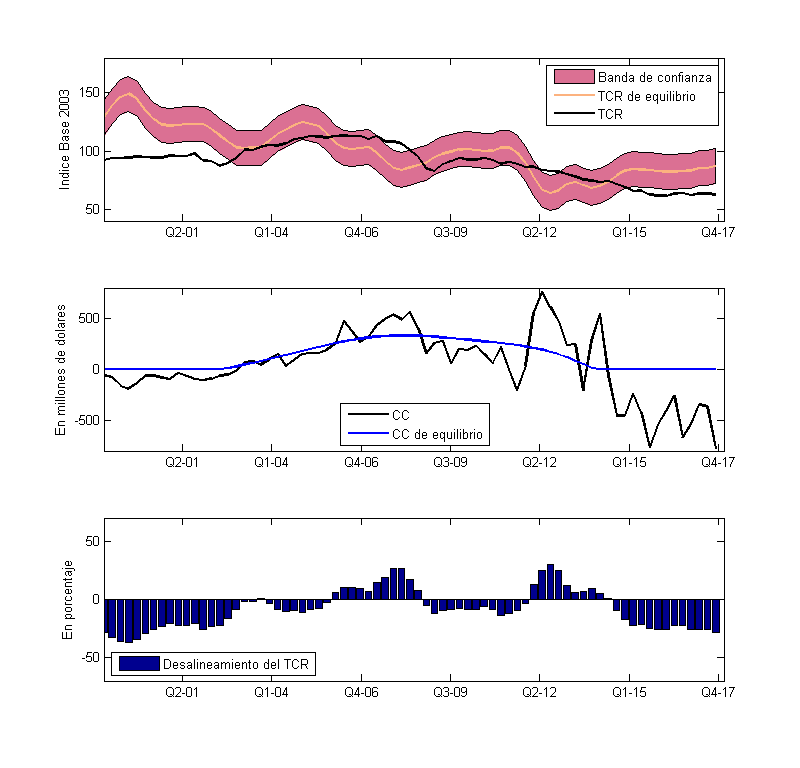
\includegraphics[scale=0.41]{tcreq}
\end{figure}
\end{frame}

\section[Consideraciones]{Heterodoxia}
\subsection[Contrabando]{Contrabando}
\begin{frame}{Con importaciones legales}
\begin{equation}\label{tcrlog}
q_t=e_t+p_t^*-p_t.
\end{equation}
\begin{align}
&p^*=\alpha p_N^*+(1-\alpha)[\beta p_{Td}^*+(1-\beta)p_{Ti}^*],\\
&p=\alpha p_N+(1-\alpha)[\beta p_{Td}+(1-\beta)p_{Ti}],
\end{align}
\begin{equation}\label{mark}
q=q_{Tl}+\alpha (\hat{p}_{N} - \hat{p}_{Tl}),
\end{equation}
Donde $q_{Tl}=e+p_{Tl}-p_{Tl}^*$. 
\end{frame}

\begin{frame}{Con contrabando}
\begin{align}
&p^*=\alpha p_N^*+(1-\alpha)[\beta p_{Td}^*+(1-\beta)p_{Ti}^*],\\
&p=\alpha p_N+(1-\alpha)\{\beta p_{Td}+(1-\beta)[\delta p_{Tii} + (1-\delta)p_{Til}]\},
\end{align}
\begin{equation}\label{contra}
q=q_{Tl}+\alpha (\hat{p}_{N} - \hat{p}_{Tl}) + (1-\alpha)(1-\beta)\delta (p_{Til}-p_{Tii}),
\end{equation}
Donde $p_{Tl}=\beta p_{Td}+(1-\beta)p_{Til}$.\\
$p_{Til}-p_{Tii}>0$
\end{frame}

\begin{frame}{Con contrabando en ambos economías}
\Wider{\begin{align}
&p^*=\alpha p_N^*+(1-\alpha)\{\beta^* p_{Td}^*+(1-\beta^*)[\delta^* p_{Tii}^* + (1-\delta^*)p_{Til}^*]\},\\
&p=\alpha p_N+(1-\alpha)\{\beta p_{Td}+(1-\beta)[\delta p_{Tii} + (1-\delta)p_{Til}]\}.
\end{align}
Donde: $\beta \neq \beta^*$ y $\delta \neq \delta^*$.
\begin{align*}
q=&q_{Tl}+\alpha (\hat{p}_{N} - \hat{p}_{Tl}) \\\nonumber &+ (1-\alpha)[(1-\beta^*)\delta^* (p_{Tii}^*-p_{Til}^*)-(1-\beta)\delta (p_{Tii}-p_{Til})].
\end{align*}
Considérese que tanto $p_{Tii}^*-p_{Til}^*<0$ como $p_{Tii}-p_{Til}<0$}
\end{frame}

\subsection[Organización industrial]{Organización industrial}
\begin{frame}{Cournot y Bertrand}
\begin{itemize}
\item Competencia à la Cournot en la que todos los productos son perfectos sustitutos. \item La solución del modelo indica que se obtiene un solo precio de equilibrio. 
\item La demanda total es atendida por todos los competidores siendo que el sector más eficiente se queda con la mayor parte de los requerimientos de bienes y la menos eficientes con la menor proporción del mercado. 
\item Modelo de competencia de Bertrand en el que sólo los sectores más eficientes o con menor costo marginal sobreviven a una competencia de precios.
\end{itemize}
\end{frame}

\begin{frame}{Hotelling y Salop}
\begin{itemize}
\item Distinguir que los productos son diferenciados horizontalmente, en este caso el modelo Hotelling (y Salop).
\item Determina que mientras más cerca esté el productor del consumidor mayor demanda podrá acaparar en un área de proximidad determinado por la cercanía de sus competidores.
\item Implica que en este caso la homogeneidad de los productos (perfecta sustituibilidad) es deseable para lograr la división de la demanda entre competidores. 
\end{itemize}
\end{frame}

\begin{frame}{Hotelling diferenciado}
\begin{itemize}
\item Diferenciación vertical, es decir que los productos son diferenciados por su calidad, siendo que los consumidores prefieren los bienes de mejor calidad. 
\item El modelo modificado de Hotelling para este caso indica que la demanda procurará productos de mayor calidad dependiendo de su restricción presupuestaria.
\item La razón es que la solución del modelo predice que los artículos de mayor calidad tendrán un precio más elevado y una proporción del mercado relativamente baja.
\item Para poder maximizar la competencia oligopolística se realiza la diferenciación vertical de su oferta para que cada demandante escoja la calidad de bien que le convenga.
\end{itemize}
\end{frame}

\subsection[Política]{Política}
\begin{frame}
\begin{figure}
\centering
        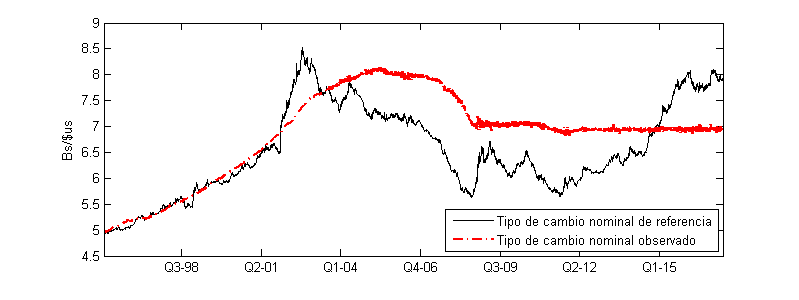
\includegraphics[width=\textwidth]{tcn}
        \label{tcn}
\end{figure}
\end{frame}

\begin{frame}{Si existe pass-through}
Dependiendo del nivel de \emph{pass-through}, considérese:
\begin{equation}
Q_t=E_t\frac{P_t^*}{P_t(E_t)},
\end{equation}
Donde, en niveles de \emph{pass-through} completos el tipo de cambio real únicamente depende del nivel de precios externo.
\end{frame}




\end{document}
